\chapter{Resultados e produtos obtidos}
\label{ch:4}

\section{Software final}
O conjunto de ferramentas analíticas desenvolvidas nesse trabalho para auxiliar a tomada de decisões da pró-reitoria
de pós-graduação da USP, recebeu o nome de DataUSP-PósGrad.
\par Sua primeira versão foi lançada oficialmente no dia 05 de junho de 2013, bem recebida pela
comunidade de gestores dos programas de pós-graduação da USP. Ganhou uma matéria na revista \emph{Espaço Aberto} da USP, nas edições 152 e 153\footnote{DataUSP-PósGrad na revista Espaço Aberto - \url{http://espaber.uspnet.usp.br/espaber/?materia=usp-desenvolve-sistema-analitico-de-dados}}.
\par Para capacitar os usuários e apresentar as ferramentas em detalhes, foram realizadas duas oficinas em todos os campus da USP, uma logo após o lançamento~\footnote{1ª oficina DataUSP-PósGrad - \url{http://iptv.usp.br/portal/home.jsp?tipo=0\&\_InstanceIdentifier=0\&\_EntityIdentifier=uspJ3kF6s9CQwQPddjpvikTCs\_sbQicdp
54HCw6bnX8bJs.\&idRepositorio=0\&modelo=0 }} e a segunda na última semana de novembro de 2013.
\par O sistema pode ser acessado por meio do portal \emph{uspdigital} no endereço \emph{http://uspdigital.usp.br/datausppg}. Por disponibilizar informações sensíveis dos programas e dos docentes da USP, o sistema pode ser acessado apenas por um grupo restrito de usuários (Dirigentes de unidades e seus secretários, Reitor, Pró-reitores e alguns outros). Além disso as bases de dados são acessíveis somente de alguns endereços ip específicos, administrados pelo Departamento de Informática da USP.
\par Pelos motivos descritos acima, e também por direitos de produção intelectual, o código do DataUSP-PósGrad pertencente à Pró-Reitoria de Pós-Graduação. O software produzido está em fase de registro pela Diretoria de Informática da Universidade de São Paulo e, uma vez registrado, deverá ser disponibilizado publicamente em forma de serviços.

\section{Teste de Carga}

Algumas consultas aos bancos de dados para gerar os relatórios no DataUSP-PósGrad são expressivamente caras computacionalmente, ou seja, um grande volume de dados precisa ser processado para se obter o resultado. Isso se traduz em tempo de processamento e, por consequência, o usuário do sistema precisa esperar alguns segundos para poder visualizar os dados. Com isso foram elaborados alguns teste de carga, com a finalidade de aferir o tempo de resposta do sistema simulando uma certa quantidade de usuários simultâneos e, poder avaliar a usabilidade como também a sensação de fluidez de DataUSP-PósGrad em uma situação de alta demanda.

\subsection{Metodologia de teste}

Os testes foram realizados com o relatório de Titulações por Ano~\ref{subsub:titano}(Ilustrado no exemplo~\ref{sub:exemplo}). Para cada usuário simulado é sorteada aleatoriamente uma área da pós-graduação para a qual deseja-se exibir o relatório do numero de títulos por ano, no intervalo de 1970 a 2013, do mesmo modo que seria feito utilizando-se a Interface Web. Os resultados são uma média de três repetições de cada teste.
\par
Foram utilizados dois bancos de dados distintos: Sybase ASE versão 13, que é utilizado em produção pelo DataUSP-PósGrad e também pelos demais sistemas administrativos da USP; Microsoft SQL Server versão 11, utilizado para armazenar o modelo multi-dimensional~\ref{sub:multi} e gerar os cubos off-line. 
\par
Para simular a carga de usuários foi utilizado o software JMeter~\footnote{Apache JMeter - http://jmeter.apache.org/}. Além disso, tanto o Servidor de Recursos quanto a Interface Web do DataUSP-PósGrad foram executados na mesma máquina em todos os testes.
\par
O JMeter (figura~\ref{fig:jmeter}) é um software livre da fundação Apache escrito em Java especialmente para realizar testes de carga, aom suporte a diversos tipos de protocolos de rede e dentre eles o HTTP. No caso do DataUSP-PósGrad, o JMeter funciona executando um script que simula as ações de um usuário interagindo com a Interface Web. Esse script pode então ser executado em paralelo simulando um determinado número de usuários. O resultado é um gráfico que exibe a vazão de dados, média, mediana e desvio padrão do tempo de resposta das requisições ao Servidor de Recursos. 
\par
O objetivo desse teste é determinar o impacto da quantidade de usuários simultâneos no desempenho geral do sistema. Atualmente o DataUSP-PósGrad possui cerca de 2000 usuários cadastrados.

\begin{figure}[H]
    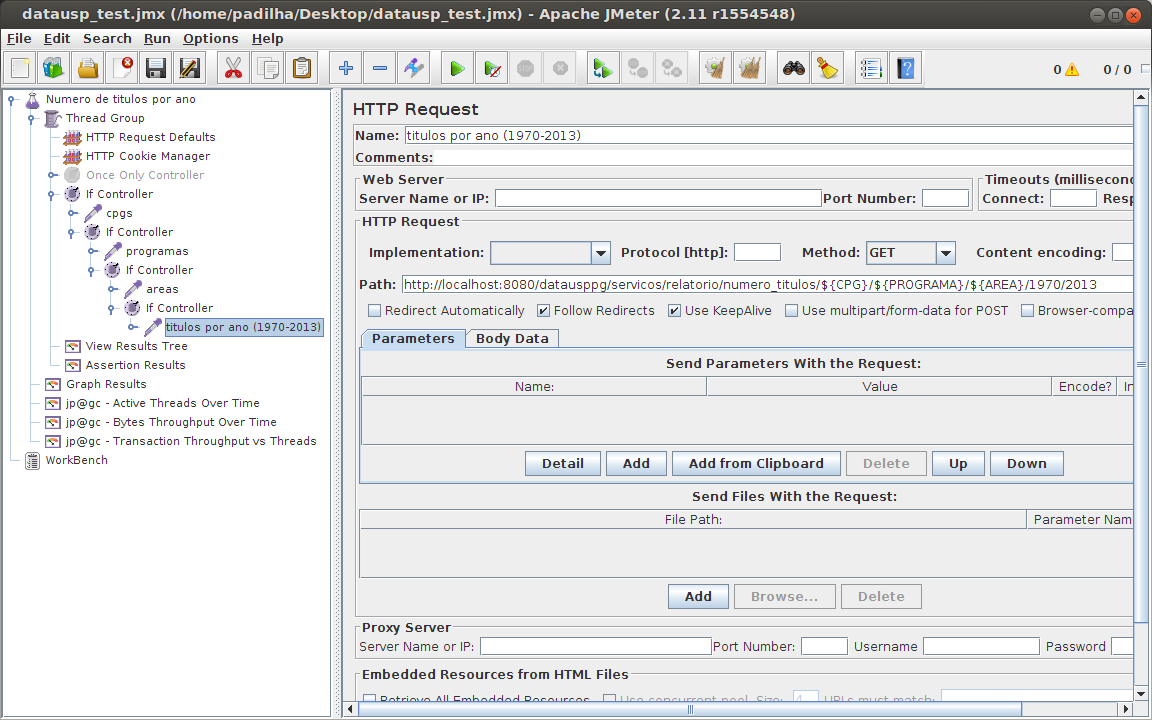
\includegraphics[width=\textwidth]{figuras/jmeter}
    \caption{Interface gráfica do JMeter}
    \label{fig:jmeter}
\end{figure}

\subsection{Resultado dos testes}

Utilizando o banco de dados Sybase ASE foram feitos testes simulando 30, 90 e 360 usuários simultâneos. Os resultados são apresentados nas figuras a seguir.

\begin{figure}[H]
\centering
\subfloat[Sybase ASE]{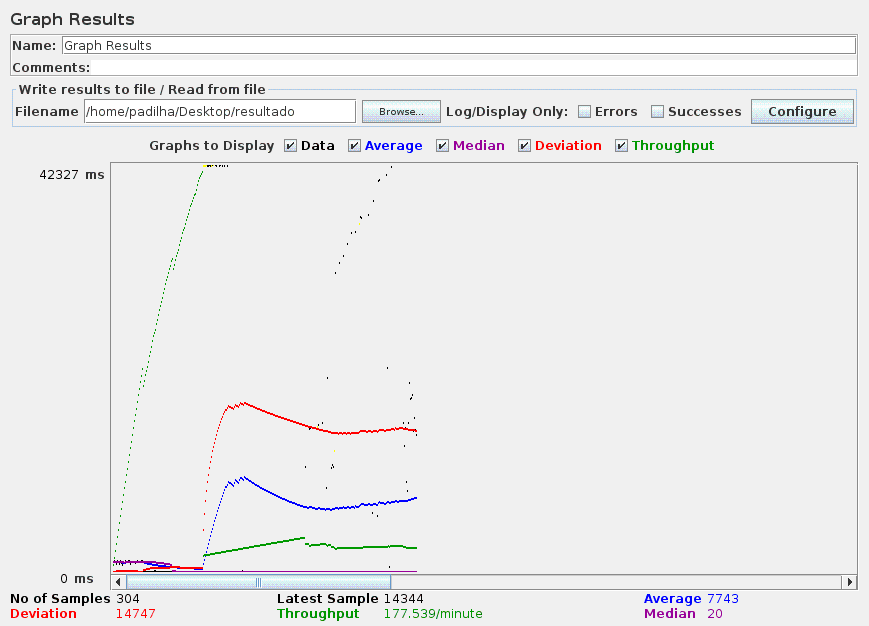
\includegraphics[width=\textwidth]{figuras/psy_30}}\\
\subfloat[MS SQL Server]{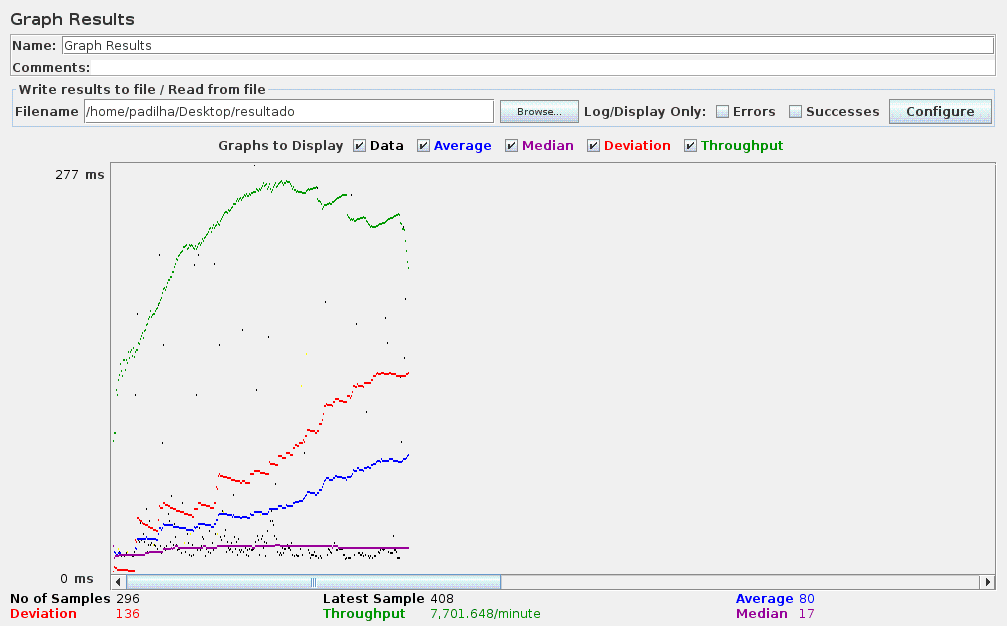
\includegraphics[width=\textwidth]{figuras/pms_30}}
\caption{Gráfico gerado pelo JMeter: 30 usuários}
\label{fig:comp_30}
\end{figure}

\begin{figure}[H]
\centering
\subfloat[Sybase ASE]{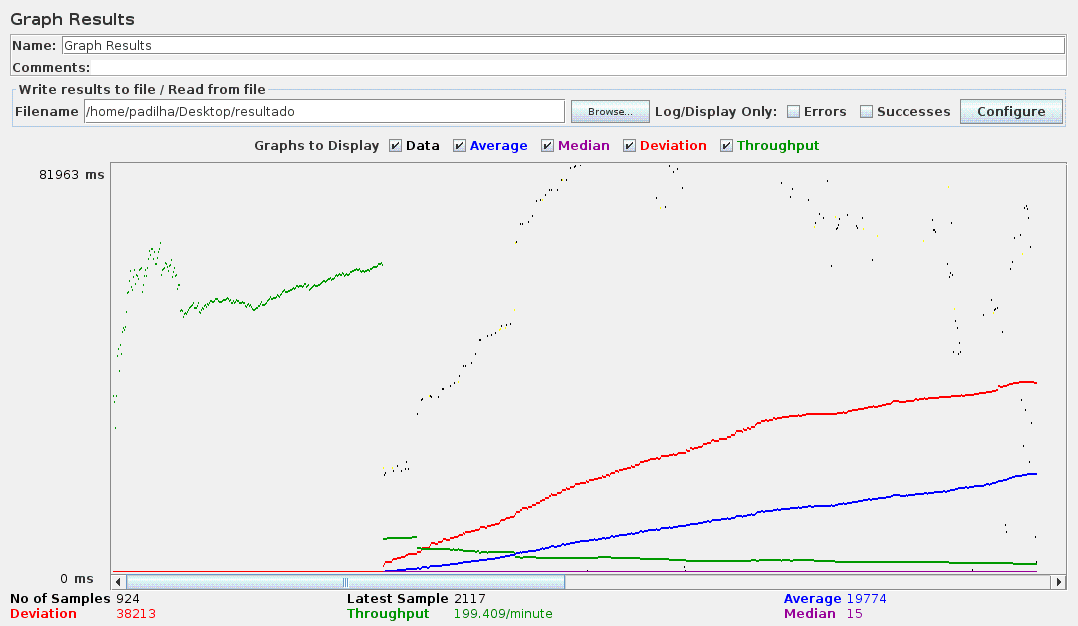
\includegraphics[width=\textwidth]{figuras/psy_90}}\\
\subfloat[MS SQL Server]{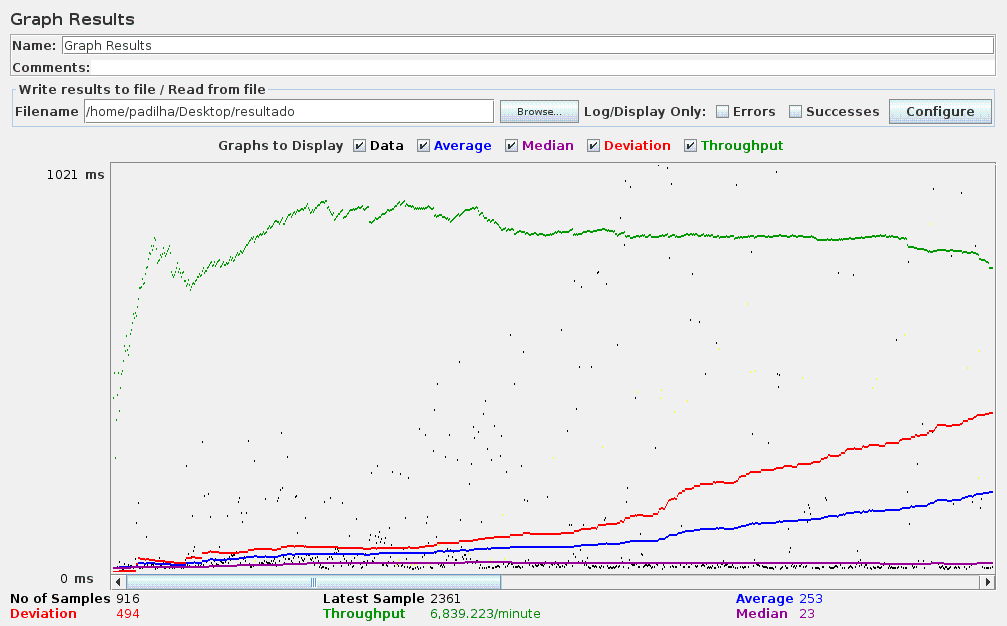
\includegraphics[width=\textwidth]{figuras/pms_90}}
\caption{Gráfico gerado pelo JMeter: 90 usuários}
\label{fig:comp_90}
\end{figure}

\begin{figure}[H]
\centering
\subfloat[Sybase ASE]{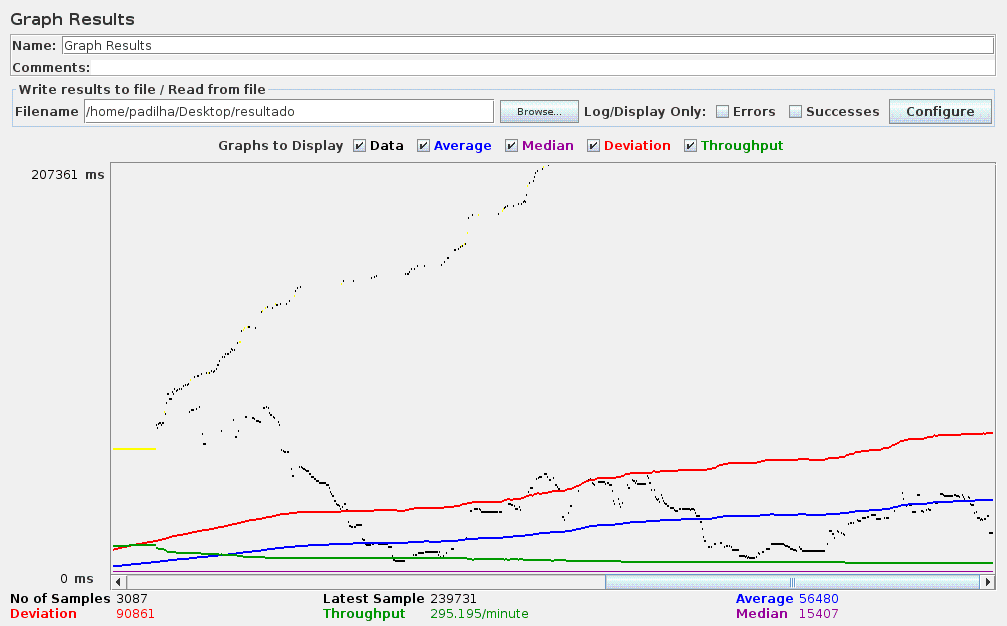
\includegraphics[width=\textwidth]{figuras/psy_360}}\\
\subfloat[MS SQL Server]{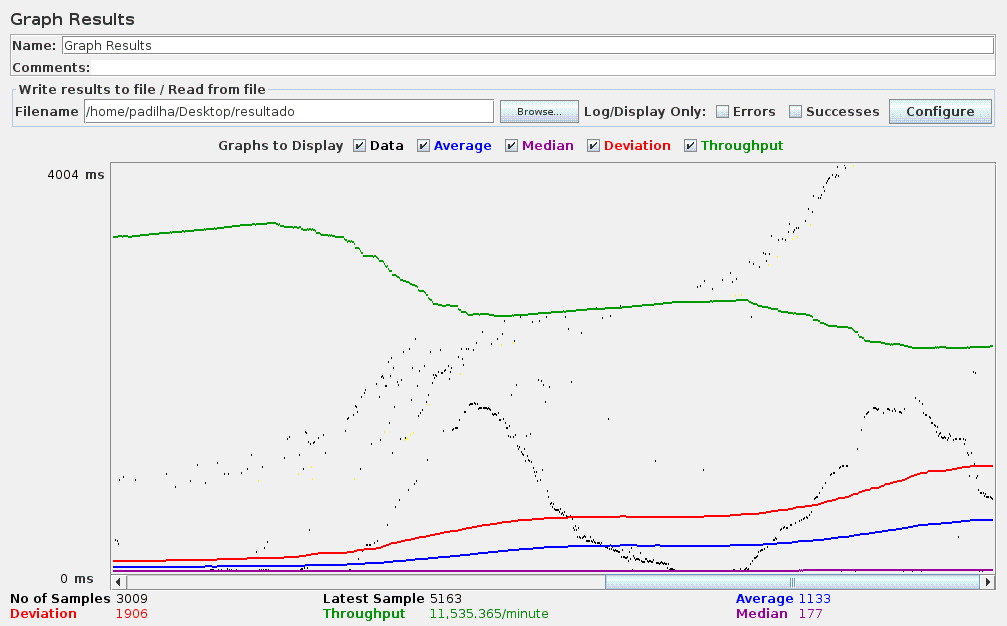
\includegraphics[width=\textwidth]{figuras/pms_360}}
\caption{Gráfico gerado pelo JMeter: 360 usuários}
\label{fig:comp_360}
\end{figure}


A linha verde nos gráficos indica a vazão de dados do servidor em transações por minuto, enquanto que as linhas vermelha, azul e lilás correspondem respectivamente ao desvio padrão, média e mediana do tempo de resposta das requisições.
\par

Analisando o tempo médio aproximado de resposta das requisições, tem-se que:

\begin{itemize}
\item 30 usuários~\ref{fig:comp_30}: 7,7s em Sybase e 80ms em MS SQL Server;
\item 90 usuários~\ref{fig:comp_90}: 19,7s em Sybase e 253ms em MS SQL Server;
\item 30 usuários~\ref{fig:comp_360}: 56,5s em Sybase e 1100ms em MS SQL Server;
\end{itemize}

\subsection{Conclusão dos testes}

Ao utilizar o banco de dados Sybase ASE no DataUSP-PósGrad não foi possível avaliar a escalabilidade dos Serviços Web REStful, uma vez que o Servidor de Recursos passou a maior parte do tempo ocioso, esperando dados do banco. Porém, ao utilizar-se o banco de dados Microsoft SQL Server que, apesar de na USP ser um banco de testes executado em uma máquina virtual, foi centenas de vezes mais rápido do que o Sybase ASE, fazendo com que o Servidor de Recursos esgotasse o processamento e também a memória ram da máquina onde foi executado nos testes.
\par
Não apenas o tempo de resposta das requisições foi consideravelmente menor no Microsoft SQL Server, como sua vazão de dados foi milhares de vezes maior, aumentando conforme o número de usuários simultâneos. O Sybase ASE, do contrário, manteve sua vazão ao longo de todos os testes, saturando sua capacidade com apenas 30 usuários simultâneos. 
\par
Apenas a título de curiosidade, foi feito um teste com dois mil usuários simultâneos (um pouco mais do que todos os usuários com acesso ao sistema). Com o Microsoft SQL Server o tempo médio de resposta do Servidor de Recursos foi de 5,2s. Ao utilizar o Sybase ASE não foi possível completar o teste pois, após alguns minutos de espera, o banco de dados repentinamente encerrava a conexão.
\par 
O uso do banco de dados Sybase ASE no DataUSP-PósGrad acarreta sérios problemas de desempenho em um cenário de alta demanda por seus serviços. Mesmo assim é o banco padrão de praticamente todos os outros sistemas administrativos da USP.
